\documentclass[11pt]{beamer}
\usetheme{Boadilla}
\usepackage[utf8]{inputenc}
\usepackage[spanish]{babel}
\usepackage{amsmath}
\usepackage{amsfonts}
\usepackage{amssymb}
\usepackage{graphicx}
\usepackage{subfig}
\usepackage{natbib}

%%%%% Color institucional
\definecolor{MyBackground}{rgb}{1.0000,0.9451,0.6549}
\definecolor{itesm}{HTML}{0658a6}
\definecolor{lnppdos}{RGB}{59,124,188}
\definecolor{lnpptres}{RGB}{124,172,212}
%\definecolor{MyBackground}{RGB}{255,241,167}
%\setbeamercolor{background canvas}{bg=MyBackground}
\setbeamercolor*{palette primary}{bg=lnpptres, fg = black}
\setbeamercolor*{palette secondary}{bg=lnppdos, fg = white}
\setbeamercolor*{palette tertiary}{bg=itesm, fg = white}
\setbeamercolor{frametitle}{fg=itesm,bg=white}
\setbeamercolor{title}{fg=white,bg=itesm}
\setbeamercolor{caption name}{fg=itesm}
\setbeamercolor*{item}{fg=itesm}

\usepackage{xcolor}
\usepackage{hyperref}

\hypersetup{
  colorlinks,
  citecolor=lnppdos,
  urlcolor=blue}

\newtheorem{recetabayesiana}{\textit{La única receta de la inferencia bayesiana...}}


%%%%%% ---------------------------------------------
%%%%%% PARA EL ALGORITMO
%%%%%% -----------------------------------------

%%%%%%%%%%%%%%%%%%%%%%%%%%%%%%


%% Para agregar el algoritmo
\usepackage[linesnumbered,ruled,vlined]{algorithm2e}
%\usepackage{algorithm2e}
\usepackage{algorithmic}

\usepackage{multicol}
\SetKwInput{KwInput}{Input}                % Set the Input
\SetKwInput{KwOutput}{Output}              % set the Output

% Para eliminar la numeración del algoritmo
%\makeatletter
%\newcommand{\RemoveAlgoNumber}{\renewcommand{\fnum@algocf}{\AlCapSty{\AlCapFnt\algorithmcfname}}}
%\newcommand{\RevertAlgoNumber}{\algocf@resetfnum}
%\makeatother
% Para comentarios azulitos
\newcommand\mycommfont[1]{\footnotesize\ttfamily\textcolor{blue}{#1}}
\SetCommentSty{mycommfont}
% Para el do n times
\SetKwFor{RepTimes}{do}{times}{end}
% Para no poner numeración en una línea en específico
\let\oldnl\nl% Store \nl in \oldnl
\newcommand{\nonl}{\renewcommand{\nl}{\let\nl\oldnl}}% Remove line number for one line
% Para poner una línea horizontal divisoria en el algoritmo
\newcommand{\hrulealg}[0]{\vspace{2mm} \hrule \vspace{2mm}}
% Para el loop forever
 \SetKwBlock{Loop}{LoopForever}{EndLoop}
% Para el switch case
\newcommand{\SWITCH}[1]{\STATE \textbf{switch} (#1)}
\newcommand{\ENDSWITCH}{\STATE \textbf{end switch}}
\newcommand{\CASE}[1]{\STATE \textbf{case} #1\textbf{:} \begin{ALC@g}}
\newcommand{\ENDCASE}{\end{ALC@g}}
\newcommand{\CASELINE}[1]{\STATE \textbf{case} #1\textbf{:} }
\newcommand{\DEFAULT}{\STATE \textbf{default:} \begin{ALC@g}}
\newcommand{\ENDDEFAULT}{\end{ALC@g}}
\newcommand{\DEFAULTLINE}[1]{\STATE \textbf{default:} }

%% Para identar el procedimiento
\newlength\myindent
\setlength\myindent{2em}
\newcommand\bindent{%
  \begingroup
  \setlength{\itemindent}{\myindent}
  \addtolength{\algorithmicindent}{\myindent}
}
\newcommand\eindent{\endgroup}
%%%%%%%%%%%%%%%%%%%%%%%%%%%%%%

%%%%%%
<<<<<<< HEAD
\title[]{Programación probabilística y problemas inversos en ecuaciones diferenciales ordinarias}
=======
\title[Clase]{Programación probabilística y problemas inversos en ecuaciones diferenciales ordinarias}
>>>>>>> 596a0eaa24d742c54afa29986847555295bdf3f0
\institute[EGTP]{Simulación de sistemas \\ Escuela de Gobierno y Transformación Pública, ITESM} 
\date{\today} 
\subject{Resultados} 
\titlegraphic{
\includegraphics[width=3cm]{images/egap}\hspace*{7.5cm}
}
%\title{Turing ODE}
%\setbeamercovered{transparent} 
%\setbeamertemplate{navigation symbols}{} 
%\logo{} 
%\institute{} 
%\date{} 
%\subject{} 
\begin{document}

\begin{frame}
\titlepage
\end{frame}

%\begin{frame}
%\tableofcontents
%\end{frame}

\begin{frame}
	\begin{figure}
		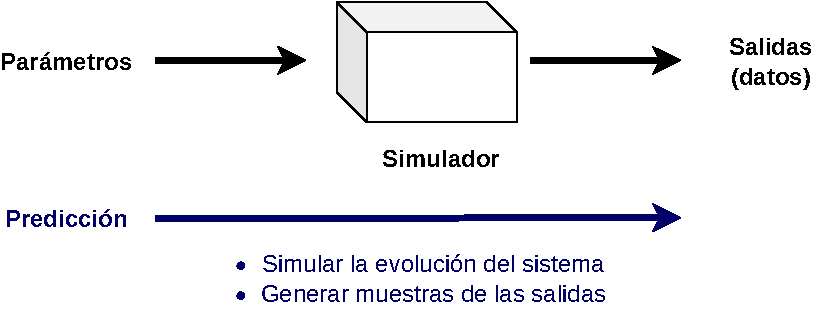
\includegraphics[scale=0.8]{images/turing_ode-simulators-1.pdf}
		\caption{\scriptsize Adaptado de Atılım Güneş Baydin, \textit{Probabilistic Programming for Inverse Problems in the Physical Sciences}. Recurso : \url{https://www.youtube.com/watch?v=E3_Ey0z068o}}
	\end{figure}
\end{frame}

\begin{frame}
	\begin{figure}
		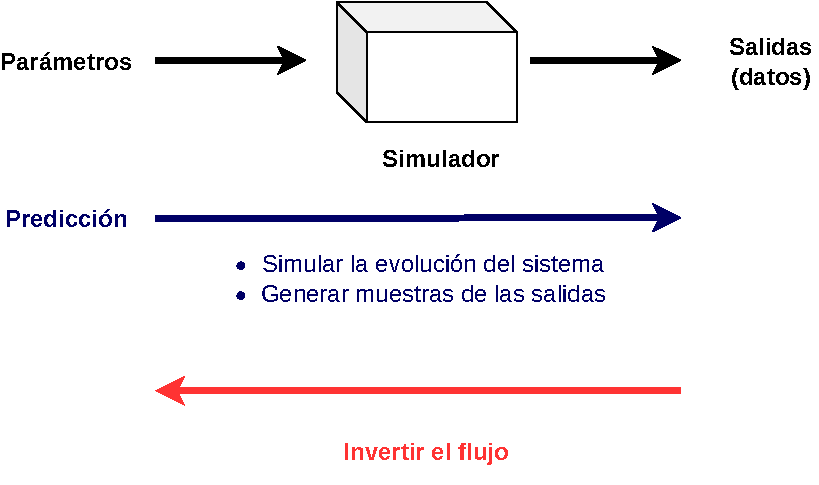
\includegraphics[scale=0.8]{images/turing_ode-simulators-2.pdf}
		\caption{\scriptsize Adaptado de Atılım Güneş Baydin, \textit{Probabilistic Programming for Inverse Problems in the Physical Sciences}. Recurso : \url{https://www.youtube.com/watch?v=E3_Ey0z068o}}
	\end{figure}
\end{frame}

\begin{frame}
	\begin{figure}
		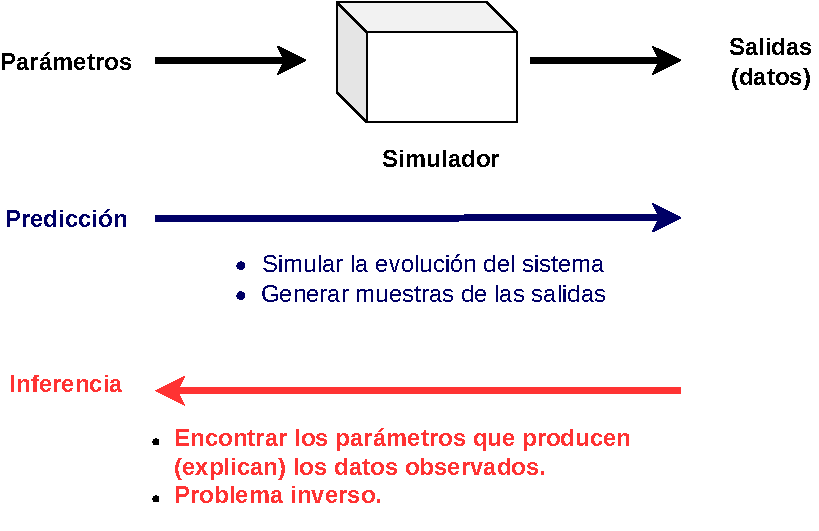
\includegraphics[scale=0.8]{images/turing_ode-simulators-3.pdf}
		\caption{\scriptsize Adaptado de Atılım Güneş Baydin, \textit{Probabilistic Programming for Inverse Problems in the Physical Sciences}. Recurso : \url{https://www.youtube.com/watch?v=E3_Ey0z068o}}
	\end{figure}
\end{frame}

\begin{frame}{Reconstrucción de redes}
	\begin{figure}
		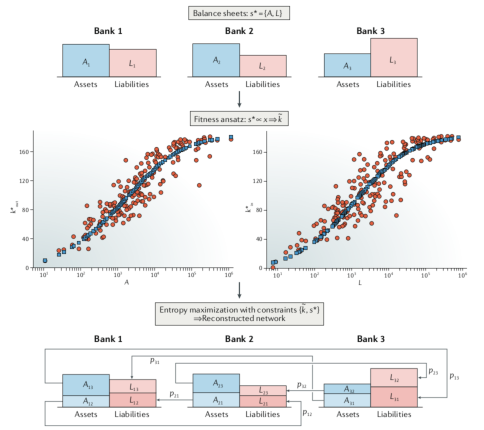
\includegraphics[scale=0.9]{images/financial_net}
		\caption{\tiny Tomado de Cimini, G., Squartini, T., Garlaschelli, D. \& Gabrielli, A Systemic risk analysis on reconstructed economic and
financial networks. Sci. Rep. 5, 15758 (2015).}
	\end{figure}
\end{frame}


\begin{frame}
	\begin{figure}
		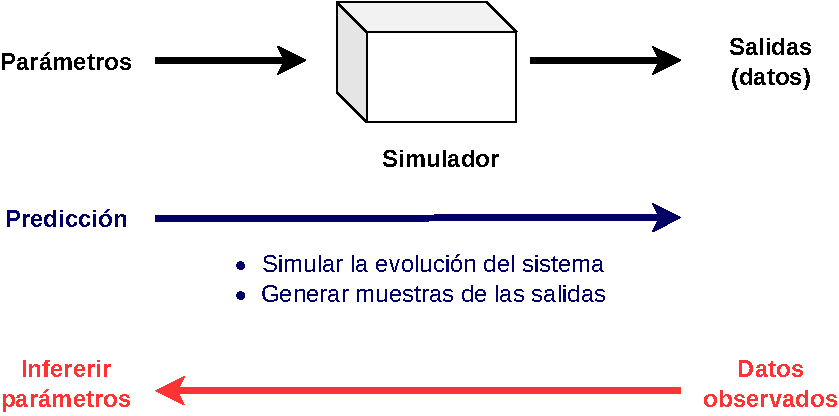
\includegraphics[scale=0.8]{images/turing_ode-simulators-4.pdf}
		\caption{\scriptsize Adaptado de Atılım Güneş Baydin, \textit{Probabilistic Programming for Inverse Problems in the Physical Sciences}. Recurso : \url{https://www.youtube.com/watch?v=E3_Ey0z068o}}
	\end{figure}
\end{frame}

\begin{frame}{Programación probabilística}
	\begin{columns}
\begin{column}{0.5\textwidth}

	\begin{itemize}
	\item Es un enfoque de aprendizaje de máquinas que permite escribir programas que representan modelos probabilísticos.
	\item La programación probabilística soporta declaraciones probabilísticas como declaración de variables aleatorias.
	\item Permite la inferencia (bayesiana) de parámetros condicionados en datos observados.
	\end{itemize}
\end{column}
\begin{column}{0.5\textwidth}
	\begin{figure}
		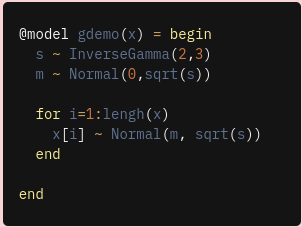
\includegraphics[scale=0.4]{images/prob_prog}
	\end{figure}
\end{column}

\end{columns}
\end{frame}

\begin{frame}{Frameworks para programación probabilística}
\begin{figure}%
 \subfloat[\centering Pyro]{{
\includegraphics[width=4cm]{images/pyro} }}%
 \qquad
 \subfloat[\centering Stan]{{
\includegraphics[width=4cm]{images/stan} }}%    \caption{2 Figures side by side}%
    \label{fig:example}%
\end{figure}
\end{frame}

\begin{frame}{Turing.jl }
	\begin{figure}
		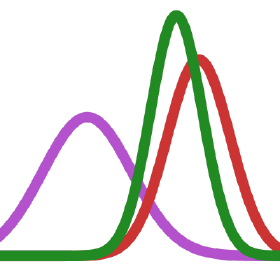
\includegraphics[scale=0.4]{images/turing}
		\caption{\url{https://turing.ml/stable/}}
	\end{figure}
\end{frame}

\begin{frame}{Julia}
	\begin{figure}
		
\includegraphics[scale=0.3]{images/julia}
	\end{figure}
\end{frame}


\begin{frame}{¿Por qué otro lenguaje de alto nivel?}


\begin{columns}
\begin{column}{0.5\textwidth}
	{\center \textbf{Características típicas}}
	
	\begin{itemize}
		\item Tipado dinámico. 
		\item Sintaxis de alto nivel.
		\item Open source.
		\item Built-in package manager.
	\end{itemize}
\end{column}
\begin{column}{0.5\textwidth}  %%<--- here
	{\center \textbf{Características novedosas}}
	\begin{itemize}
		\item Buen perfomance: tiempo de ejecución rápido (\href{https://www.youtube.com/watch?v=uecdcADM3hY&t=205s}{\scriptsize Celeste.jl : Cataloging the Visible Universe Through Bayesian Inference at Petascale in Julia}). 
		\item Compilación JIT (Just in Time) a nivel de función.
		\item En un porcentaje alto, Julia está escrito en Julia. 
		\item Metaprogramación (macros).
	\end{itemize}
\end{column}
\end{columns}

\end{frame}

\begin{frame}
	\begin{figure}
		
\includegraphics[scale=0.17]{images/raz_julia}
		\caption{\url{https://www.youtube.com/watch?v=KVnj4xuktpw&t=10s}}
	\end{figure}
\end{frame}


\begin{frame}{Ecuaciones diferenciales ordinarias\footnote{Tomado de las notas de Ben Lampert sobre inferencia bayesiana \url{https://ben-lambert.com/bayesian-short-course/}}}

Realizamos experimentos donde se inoculan placas de agar con bacterias en el tiempo 0.
	\begin{figure}
		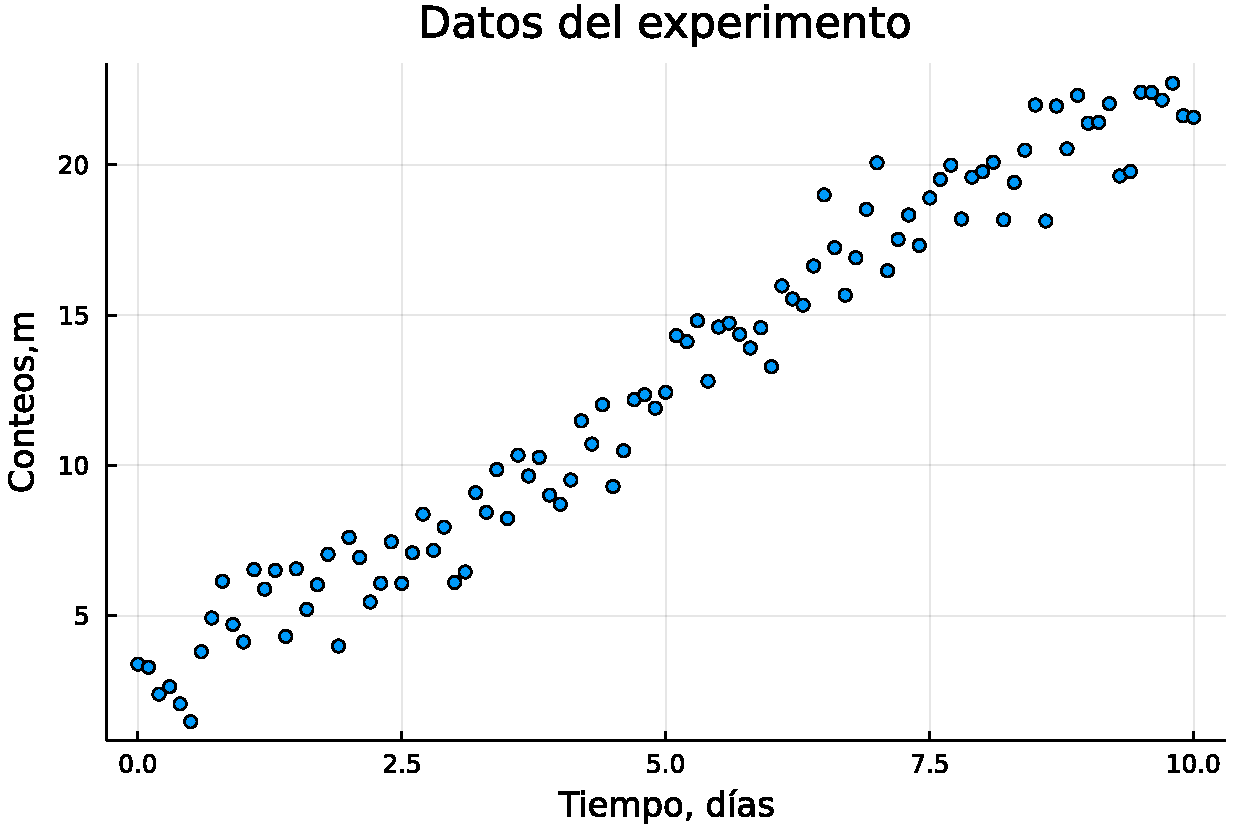
\includegraphics[scale=0.4]{images/bacterias_experimento.pdf}

	\end{figure}
\end{frame}

\begin{frame}
	\begin{itemize}
		\item Queremos modelar el crecimiento de una población de bacterias.
		\item Se asume el siguiente modelo de crecimiento poblacional,
		
		\[\dfrac{dN}{dt} = \alpha N (1-\beta N)\]
		
		donde $\alpha > 0$ es la tasa de crecimiento debida a la división celular y $\beta >0$ mide la reducción en la trasa de crecimiento debido a la aglomeración.
		
		\begin{center}
			\textbf{¿Cómo inferimos los parámetros de este modelo?}
		\end{center}
	\end{itemize}
\end{frame}

\begin{frame}
	Asumamos un error de medición alrededor del valor verdadero:
	\[N^*(t) \sim \text{normal}(N(t),\sigma)\]	
	
	donde:
		\begin{itemize}
			\item $N^*(t)$ es el conteo de bacterias en el tiempo $t$.
			\item $N(t)$ es la solución de la ODE en el tiempo $t$ (número verdadero de bacterias en la placa).
			\item $\sigma >0$ mide la magnitud del error de medición alrededor del valor verdadero.
		\end{itemize}
\end{frame}

\begin{frame}
	\begin{figure}
		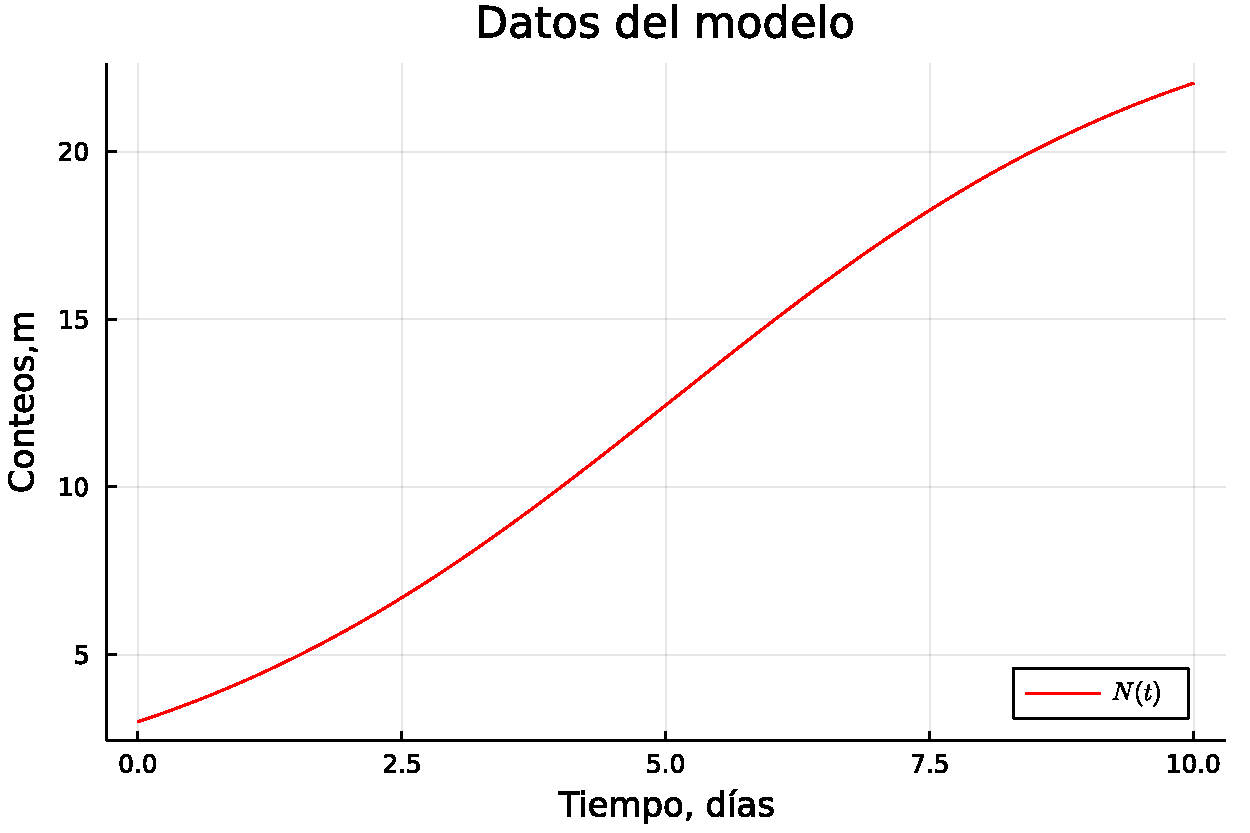
\includegraphics[scale=0.5]{images/bacterias_modelo.pdf}
		\caption{Número verdadero de bacterias, $N(t)$}
	\end{figure}
\end{frame}

\begin{frame}

Superposición de distribución de muestreo que representa el error de medición y de los datos experimentales.

	\begin{figure}
		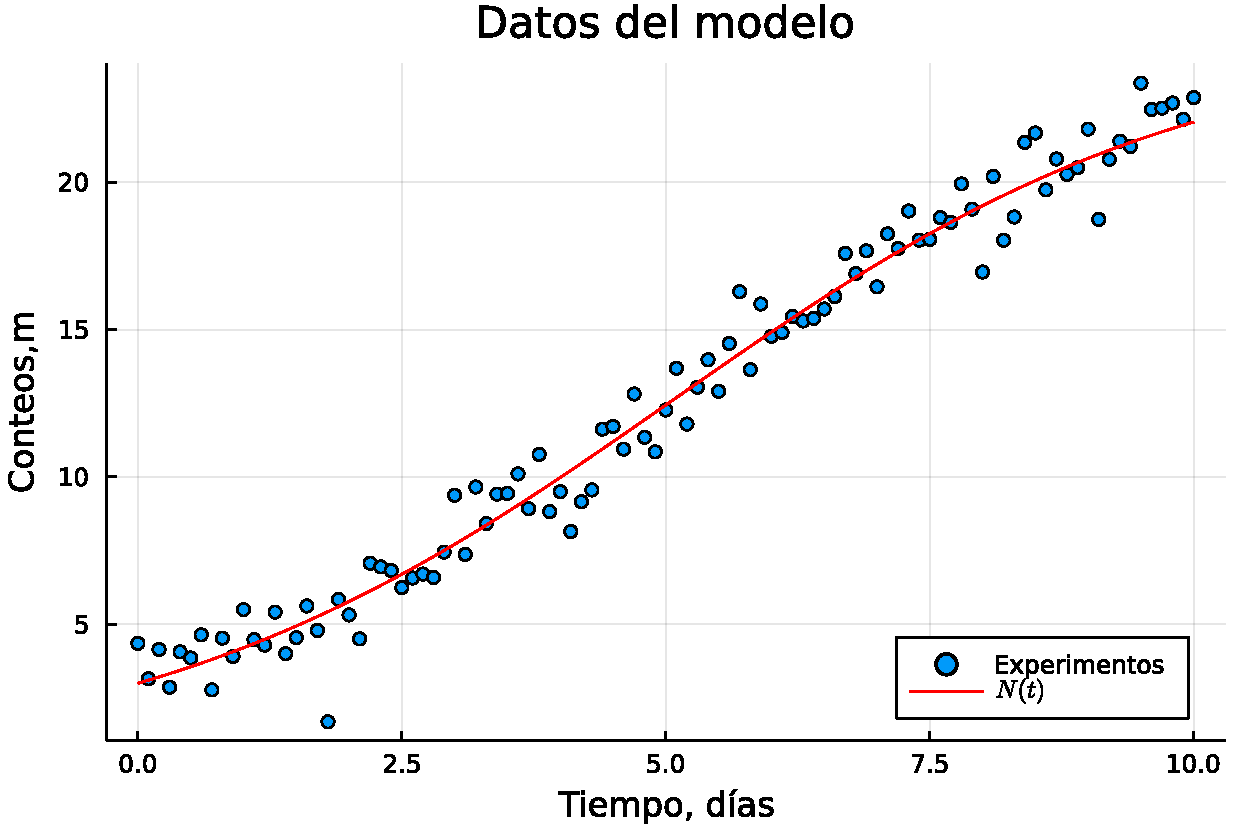
\includegraphics[scale=0.5]{images/bacterias_modelo_experimentos.pdf}
	\end{figure}
\end{frame}

\begin{frame}
%Dado que estamos usando la distribución normal,

%\[N^*(t) \sim \text{normal}(N(t),\sigma)\]

%la verosimilitud de las observaciones es

%\[L(N(t),\sigma) = \prod_{t=t_1}^T  \dfrac{1}{\sqrt{2\pi\sigma^2}} \exp{\Big[  \dfrac{-(N^*(t)-N(t))^2}{2\sigma^2}\Big]}\]

\begin{center}
	\textbf{¿Cómo calculamos $N(t)$?}
\end{center}

		\[\dfrac{dN}{dt} = \alpha N (1-\beta N)\]

\end{frame}

\begin{frame}

Cualquier solución de $N(t)$ -exacta o numérica- depende de los parámetros del modelo de ODE. En este caso,

\[N(t) = f(t,\alpha,\beta)\]

\begin{center}
	\textbf{¿Cómo integramos los datos observados para estimar estos parámetros?}
\end{center}

\end{frame}

\begin{frame}

Cualquier solución de $N(t)$ -exacta o numérica- depende de los parámetros del modelo de ODE. En este caso,

\[N(t) = f(t,\alpha,\beta)\]

\begin{center}
	\textbf{¿Cómo integramos los datos observados para estimar estos parámetros?}
\end{center}

\begin{center}
{\color{red}\huge Inferencia Bayesiana}
\end{center}

\end{frame}

\begin{frame}

Cualquier solución de $N(t)$ -exacta o numérica- depende de los parámetros del modelo de ODE. En este caso,

\[N(t) = f(t,\alpha,\beta)\]

\begin{center}
	\textbf{¿Cómo integramos los datos observados para estimar estos parámetros?}
\end{center}

\begin{center}
{\color{red}\huge Inferencia Bayesiana}
\end{center}

\begin{recetabayesiana}
consiste en encontrar la distribución condicional de todas aquellas cantidades de interés cuyo valor desconocemos dado el valor conocido de las variables observadas.
\end{recetabayesiana}
\end{frame}



\begin{frame}{Inferencia bayesiana}
	\begin{itemize}
		\item En un contexto de inferencia bayesiana, donde se tiene un modelo muestral $Y \sim p(y|\theta)$ y una distribución inicial $p(\theta)$, la distribución final se calcula de la siguiente forma:
		
		 \begin{equation*}
		 	p(\theta | y) =  \dfrac{p(y | \theta)p(\theta)}{\int p(\theta{'}) p(y|\theta{'})d\theta{'}}
		 \end{equation*} 
		\item Aún descartando el denominador (el cual se puede interpretar como un factor de escalamiento que hace que la función integre a 1), el cálculo analítico de $p(\theta | y) $, en la mayoria de las ocasiones, es complicado.
	\end{itemize}
	
\end{frame}


\begin{frame}\small
	\begin{itemize}
		\item Hay distintas técnicas para calcular $p(\theta | y) $ (aproximación de Laplace, métodos de cuadratura, etc), pero por la capacidad de cómputo disponible las técnicas de simulación de Monte Carlo vía cadenas de Markov (MCMC) han sido mayormente utilizadas.
		\item La idea de MCMC es \textbf{construir una cadena de Markov que sea fácil de simular (a través de un proceso de muestreo) y cuya distribución de equilibrio corresponda a la distribución final de interés}.
	\end{itemize}
\end{frame}

\begin{frame}
	\begin{itemize}
		\item En el contexto de nuestro problema,
		\begin{itemize}
			\item $p(\theta)$ representa la distribución inicial de los parámetros del modelo de ODE, 
			\item $p(y|\theta)$ (el modelo muestral o distribución de verosimilitud) representa el modelo de ODE. 
		\end{itemize}	
		
		\item Podemos utilizar las técnicas de MCMC para construir la distribución $p(\theta|y)$, de los parámetros del modelo de ODE.  
	\end{itemize}
\end{frame}


<<<<<<< HEAD
\begin{frame}{Método de Monte Carlo}\small

	\begin{center}
		\textbf{Idea}: Método para calcular el área bajo una curva. Es una solución estadística al problema de integración.
	\end{center}

Supongamos que existe $M > 0$ tal que $0 \leq f(\theta) \leq M$ para todo $ \theta \in [a,b]$ y que queremos calcular la integral 

	\begin{equation}
		I = \int_a^b f(\theta) d\theta
	\end{equation}

el valor de la integral es el área bajo la curva $ \phi = f(\theta)$ para $ \theta \in [a,b]$. Dicha gráfica queda inscrita en el rectángulo $R =  [a,b] \times [0,M]$.

=======
	\begin{itemize}
		\item Programación probabilística de propósito general con una interfaz de modelado intuitiva;
		\item Muestreo de Monte Carlo hamiltoniano (HMC) robusto y eficiente para distribuciones posteriores diferenciables;
		\item 
Muestreo de partículas MCMC para distribuciones posteriores complejas que involucran variables discretas y flujo de control estocástico; e
		\item 
Inferencia composicional a través del muestreo de Gibbs que combina partículas MCMC, HMC y paseo aleatorio MH (RWMH).
	\end{itemize}
>>>>>>> 596a0eaa24d742c54afa29986847555295bdf3f0
\end{frame}

\begin{frame}{Método de Monte Carlo}\small

Sea

	\begin{equation}
		p(\theta,\phi) =  \dfrac{1}{M(b-a)} I_R(\theta,\phi)
	\end{equation}
	
Entonces $p(\theta,\phi)$ corresponde a la función de densidad de una distribución uniforme sobre el rectángulo $R$. La integral $I$ puede entonces estimarse simulando una muestra $(\theta_1,\phi_1),\dots,(\theta_N,\phi_N)$ de $p(\theta,\phi)$ y contando cuántos de estos valores caen bajo la curva $ \phi = f(\theta)$.	

\vspace{0.5cm}
El estimador $\hat{I}$ obtenido es un estimador insesgado de $I$.

\vspace{0.5cm}
La varianza del estimador es 

\[Var(\hat{I}) = \dfrac{I}{N} \lbrace M(b-a) -I \rbrace\]
\end{frame}


\begin{frame}{Cálculo de $\pi$ por el método de Monte Carlo \citep{wilkinson1998}}\scriptsize

	\begin{columns}
		\begin{column}{0.5\textwidth}
			\begin{figure}
				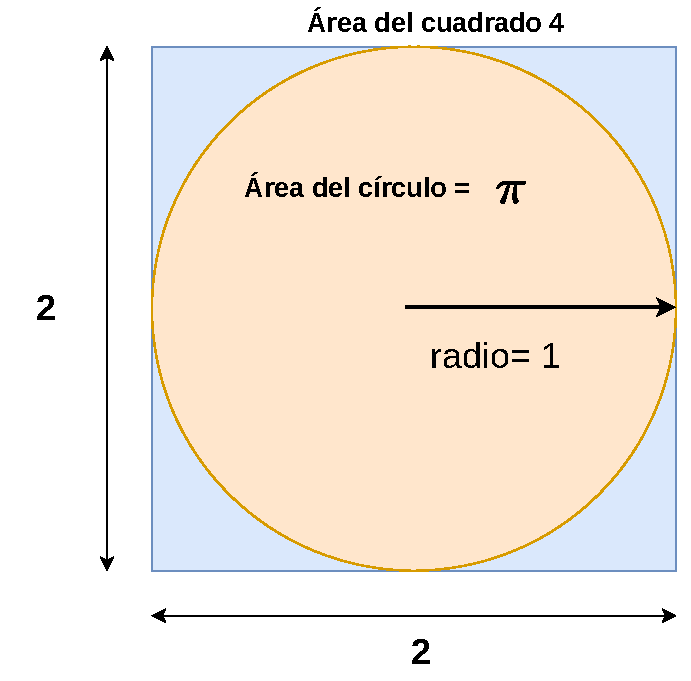
\includegraphics[scale=0.5]{images/pi-monte-carlo.pdf}
			\end{figure}
		\end{column}
		\begin{column}{0.5\textwidth}
		\[\dfrac{\text{Área del círculo}}{\text{Área del cuadrado}} = \dfrac{\pi(1)^2}{4}=\dfrac{\pi}{4}\]
		
		que puede ser descrita por la integral
		
		\[\int_0^1 \sqrt{1-x^2} dx = \dfrac{\pi}{4}\]
		
		Para calcular $\pi$ se generan parejas aleatorias de números $(x_r,y_r)$, distribuidos uniformemente entre 0 y 1, y contamos cuántos de estos puntos caen dentro del círculo, esto es, si se cumple la igualdad 
		
		\[y_r^2 + x_r^2 \leq 1\]
		\end{column}

	\end{columns}
\end{frame}

\begin{frame}
	\begin{figure}
		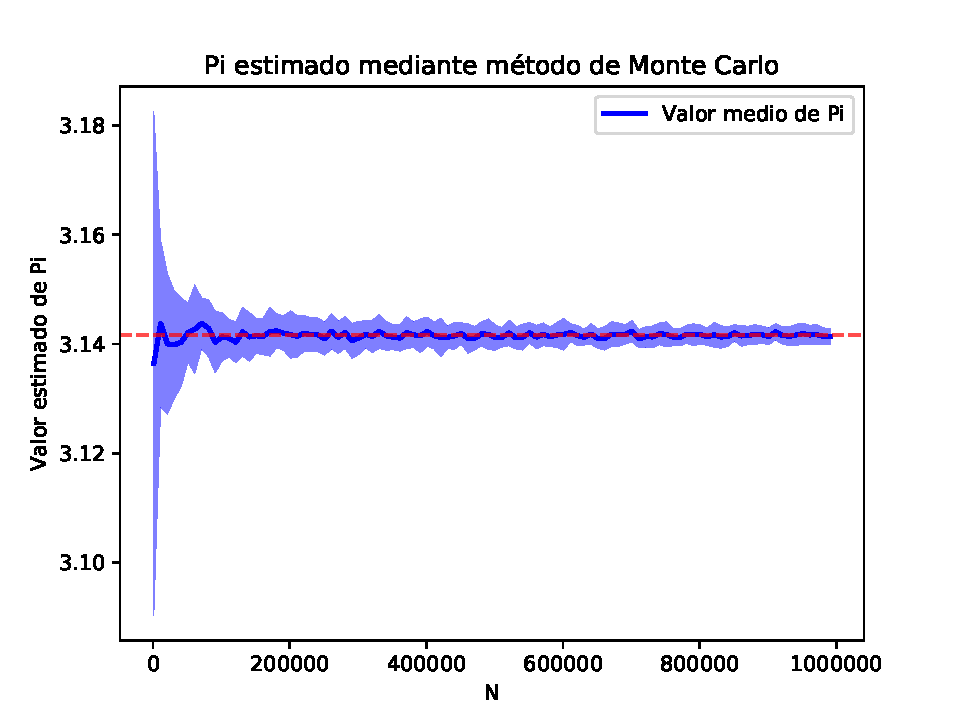
\includegraphics[scale=0.7]{images/pi_mc.pdf}
	\end{figure}
\end{frame}

\begin{frame}{Cadenas de Markov}
	
	\begin{definition} \textbf{Cadena de Markov}. Proceso estocástico discreto con estados finitos que cumple la propiedad de Markov. 

	\[P(X_{t+1} = s| X_1 = s_1, \dots ,X_t = s_t) = P(X_{t+1} = s |X_t = s_t) \]
		
	\end{definition}
	
\end{frame}

\begin{frame}{Cadenas de Markov}

			\begin{figure}
				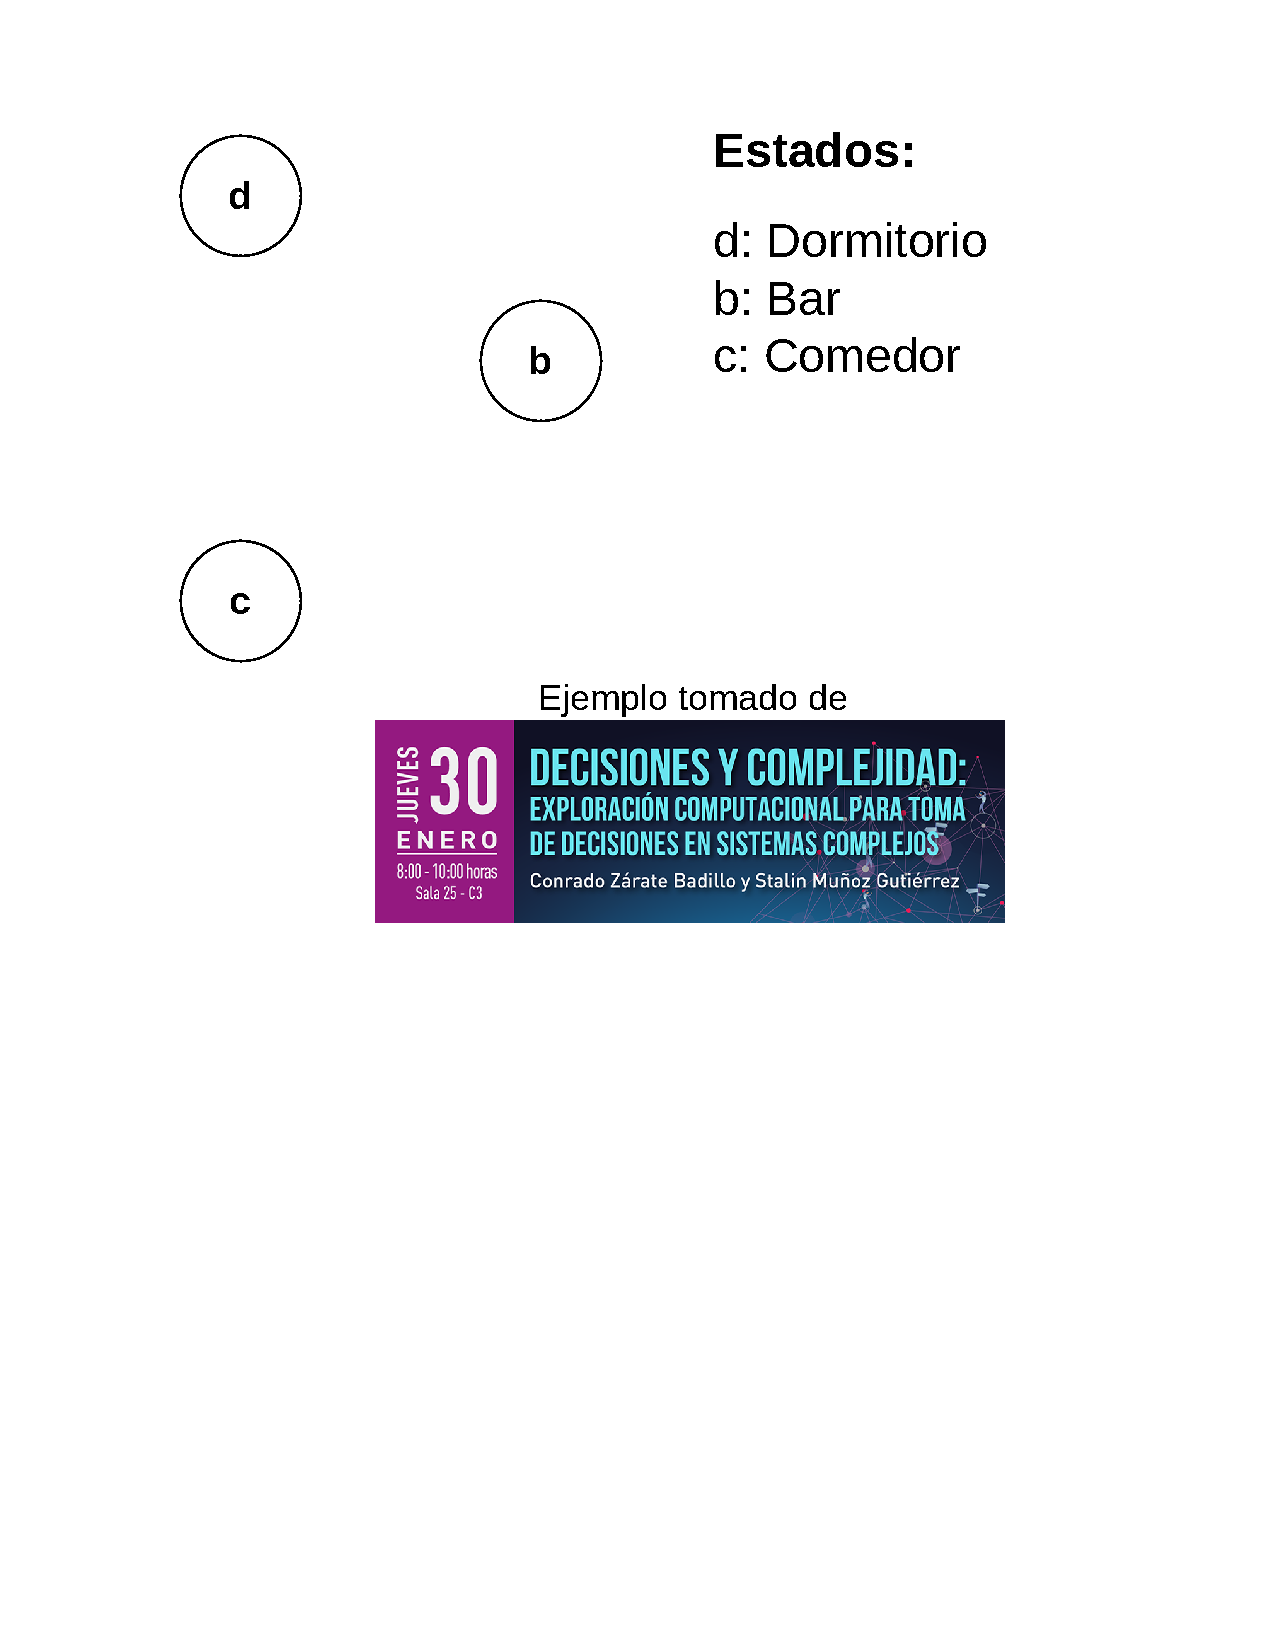
\includegraphics[scale=0.5]{images/estados.pdf}
			\end{figure}	

\end{frame}

\begin{frame}
	\begin{columns}
		\begin{column}{0.5\textwidth}
			\vspace{-0.8cm}
			\begin{figure}
				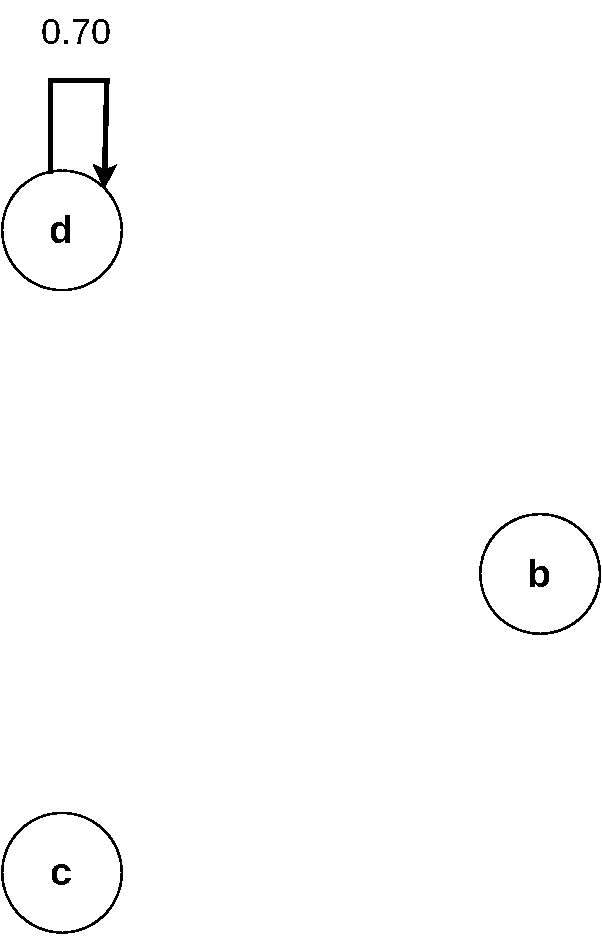
\includegraphics[scale=0.5]{images/markov_uno.pdf}
			\end{figure}
		\end{column}
		\begin{column}{0.5\textwidth}
			La arista representa la posibilidad que un pasajero que está en el dormitorio en el tiempo $t$ continúe en el dormitorio en el tiempo $t+1$.
			
			\vspace{0.5cm}
			Se etiqueta con la probabilidad de que esto suceda (\textbf{Probabilidad de transición}) 
			
			\[P(X_{t+1}´ = d \mid X_t = d)=0.7\]

		\end{column}

	\end{columns}
	
\end{frame}

\begin{frame}
	\begin{columns}
		\begin{column}{0.5\textwidth}
			\vspace{-0.8cm}
			\begin{figure}
				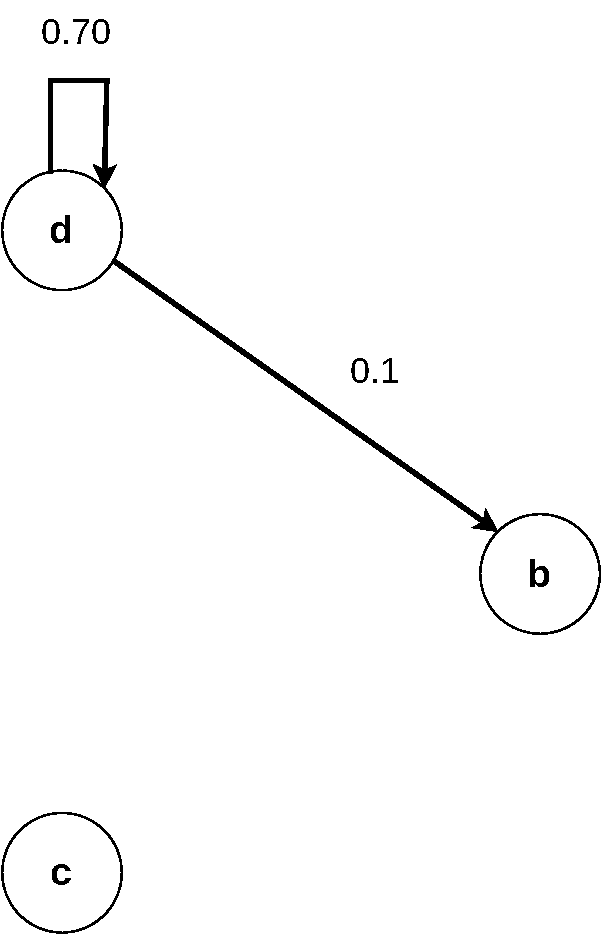
\includegraphics[scale=0.5]{images/markov_dos.pdf}
			\end{figure}
		\end{column}
		\begin{column}{0.5\textwidth}
			
		Arista para la transición del dormitorio al bar
					\[P(X_{t+1}´ = b \mid X_t = d)=0.1\]
		\end{column}

	\end{columns}
	
\end{frame}

\begin{frame}
	\begin{columns}
		\begin{column}{0.5\textwidth}
			\vspace{-0.8cm}
			\begin{figure}
				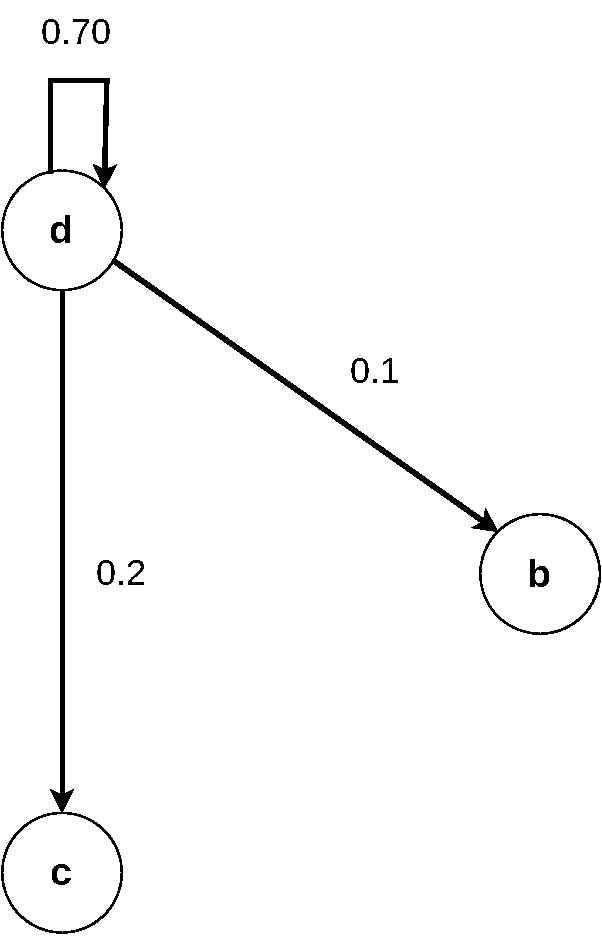
\includegraphics[scale=0.5]{images/markov_tres.pdf}
			\end{figure}
		\end{column}
		\begin{column}{0.5\textwidth}
		Arista para la transición del dormitorio al comedor
					\[P(X_{t+1}´ = c \mid X_t = d)=0.2\]
		\end{column}

	\end{columns}
	
\end{frame}

\begin{frame}
	\begin{columns}
		\begin{column}{0.5\textwidth}
			\vspace{-0.5cm}
			\begin{figure}
				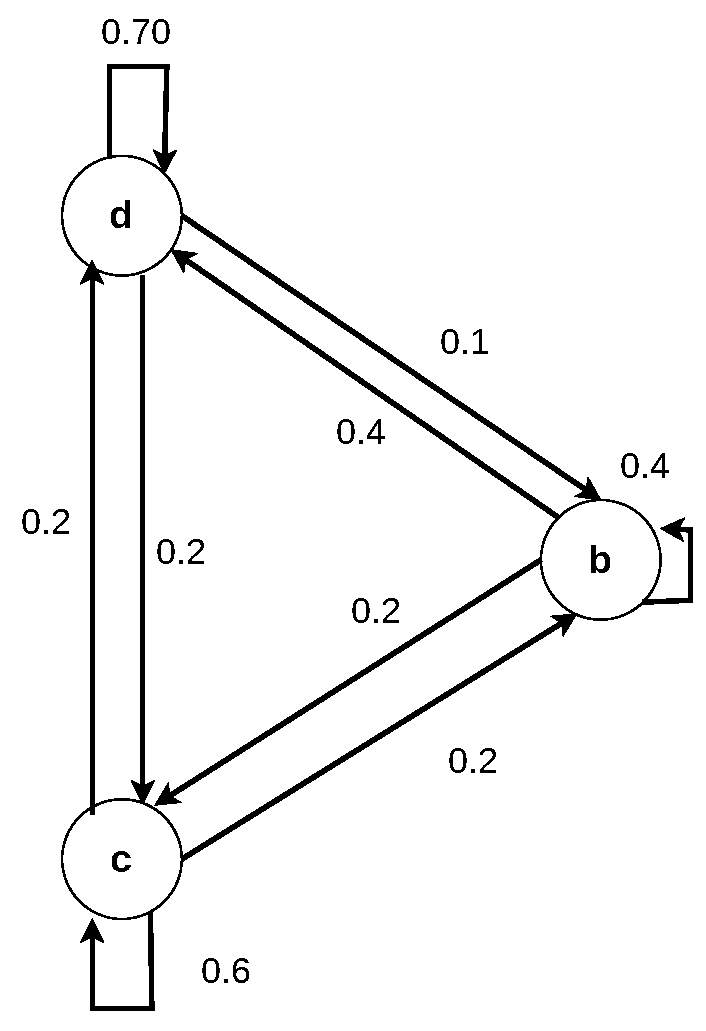
\includegraphics[scale=0.5]{images/markov_cuatro.pdf}
			\end{figure}
		\end{column}
		\begin{column}{0.5\textwidth}
			Agregamos todas las transiciones posibles y sus probabilidades.

		\end{column}

	\end{columns}
	
\end{frame}


\begin{frame}
	\begin{columns}
		\begin{column}{0.5\textwidth}
			\vspace{-0.5cm}
			\begin{figure}
				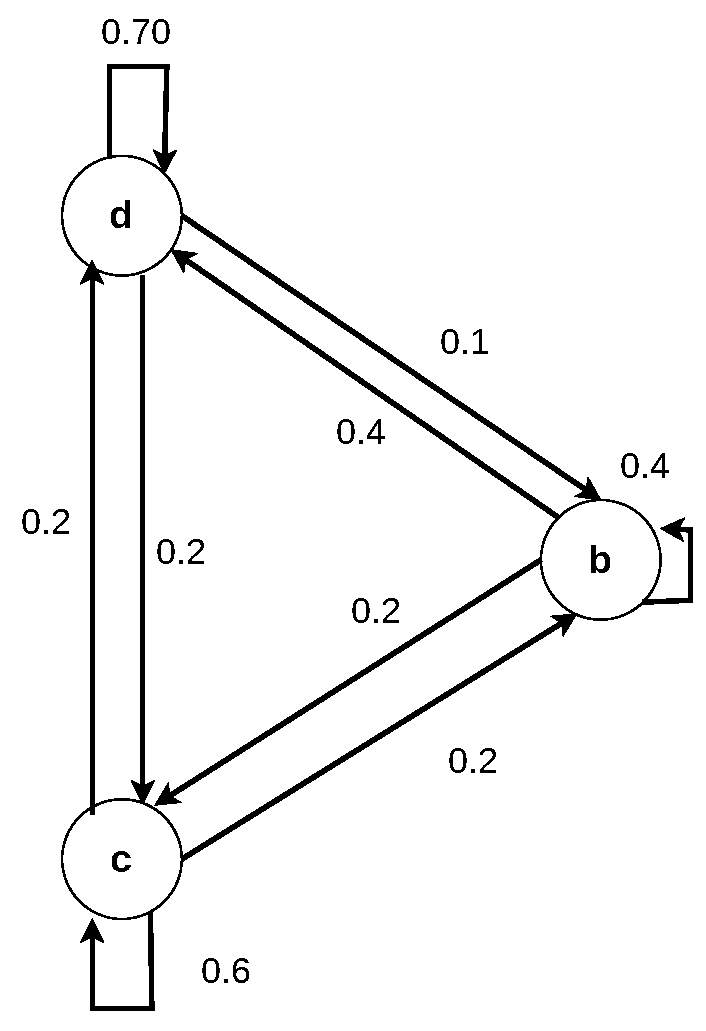
\includegraphics[scale=0.5]{images/markov_cuatro.pdf}
			\end{figure}
		\end{column}
		\begin{column}{0.5\textwidth}
			Las probabilidades de transición pueden representarse de manera matricial:
			
			\begin{equation}
			T = \begin{bmatrix}
			0.7 & 0.4 & 0.2\\
			0.1 & 0.4 & 0.2\\
			0.2 & 0.2 & 0.6
			\end{bmatrix}
			\end{equation}

			con entradas
			
			\[p_{i,j} \equiv P(X_{t+1} = i \mid X_t =j)\]

		\end{column}

	\end{columns}
	
\end{frame}

\begin{frame}
	\begin{columns}
		\begin{column}{0.5\textwidth}
			\vspace{-0.5cm}
			\begin{figure}
				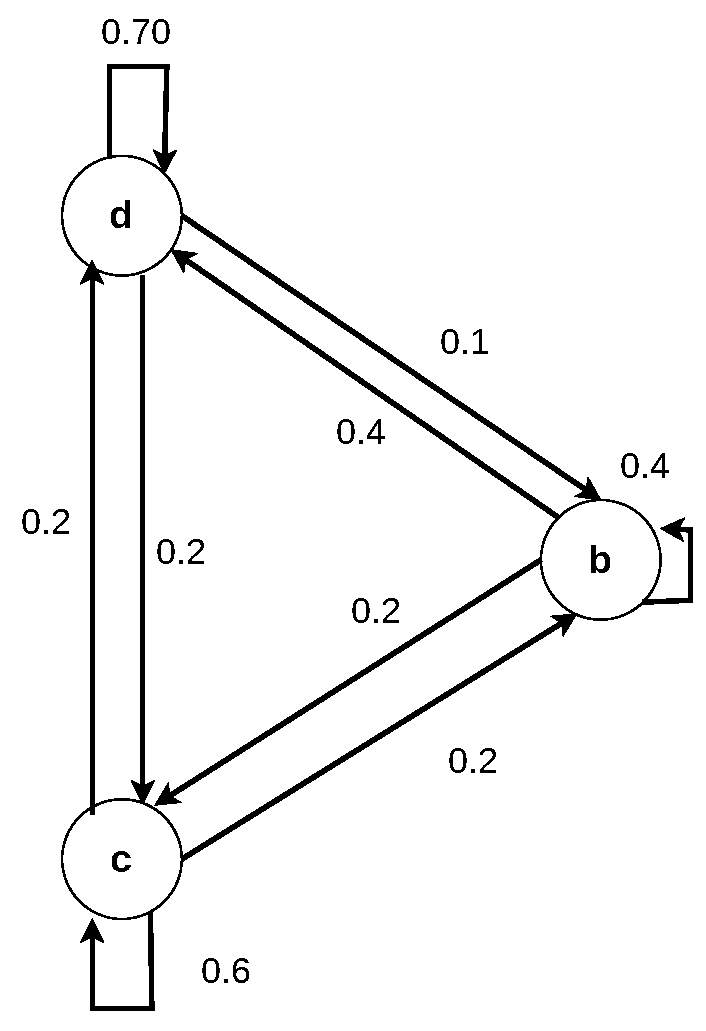
\includegraphics[scale=0.5]{images/markov_cuatro.pdf}
			\end{figure}
		\end{column}
		\begin{column}{0.5\textwidth}
			Matriz de probabilidad de estado:
			
			\begin{equation*}
			T = \begin{bmatrix}
			0.7 & 0.4 & 0.2\\
			0.1 & 0.4 & 0.2\\
			0.2 & 0.2 & 0.6
			\end{bmatrix}
			\end{equation*}

			La dinámica para la distribución de probabilidad puede expresarse:
			
			\begin{equation}
			\begin{bmatrix}
			P(X_{t+1}  = d) \\
			P(X_{t+1}  = b)\\
			P(X_{t+1}  = c) 	
			\end{bmatrix} = 
			T \begin{bmatrix}
			P(X_{t}  = d) \\
			P(X_{t}  = b)\\
			P(X_{t}  = c) 	
			\end{bmatrix}
			\end{equation}
			
			\begin{equation}
			P(X_{t+1}) = TP(X_{t})
			\end{equation}
		\end{column}

	\end{columns}
	
\end{frame}

\begin{frame}\small
	\begin{columns}
		\begin{column}{0.5\textwidth}
			\vspace{-0.5cm}
			\begin{figure}
				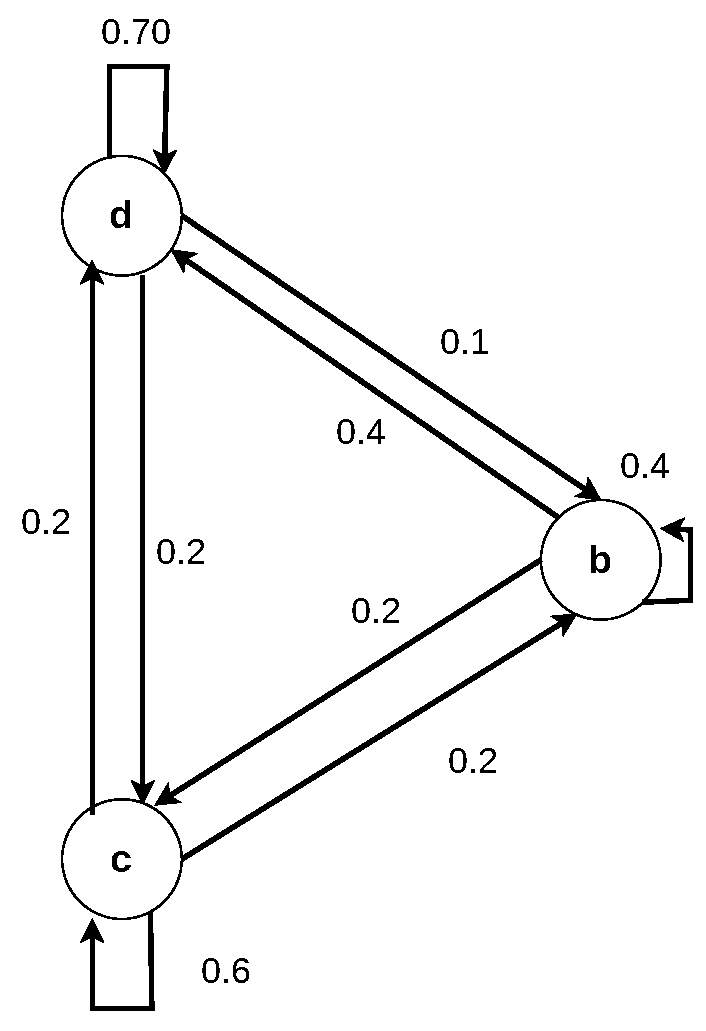
\includegraphics[scale=0.5]{images/markov_cuatro.pdf}
			\end{figure}
		\end{column}
		\begin{column}{0.5\textwidth}
			Si sabemos que el pasajero se encuentra en el dormitorio al tiempo $t = 0$:
			\[P(X_0)= \begin{bmatrix}
						1 \\
						0 \\
						0
					  \end{bmatrix}
						=P_0\]
			Al tiempo siguiente la distribución es:
			
			
			\[P(X_1) = TP_0=P_1\]
			
			\[P(X_1) = \begin{bmatrix}
			0.7 & 0.4 & 0.2\\
			0.1 & 0.4 & 0.2\\
			0.2 & 0.2 & 0.6
			\end{bmatrix} \begin{bmatrix}
						1 \\
						0 \\
						0
					  \end{bmatrix}\]
					  
			\[P(X_1) = 					  
			\begin{bmatrix}
						0.7 \\
						0.1 \\
						0.2
					  \end{bmatrix}		 \]
		\end{column}

	\end{columns}
	
\end{frame}



\begin{frame}\small
	\begin{columns}
		\begin{column}{0.5\textwidth}
			\vspace{-0.5cm}
			\begin{figure}
				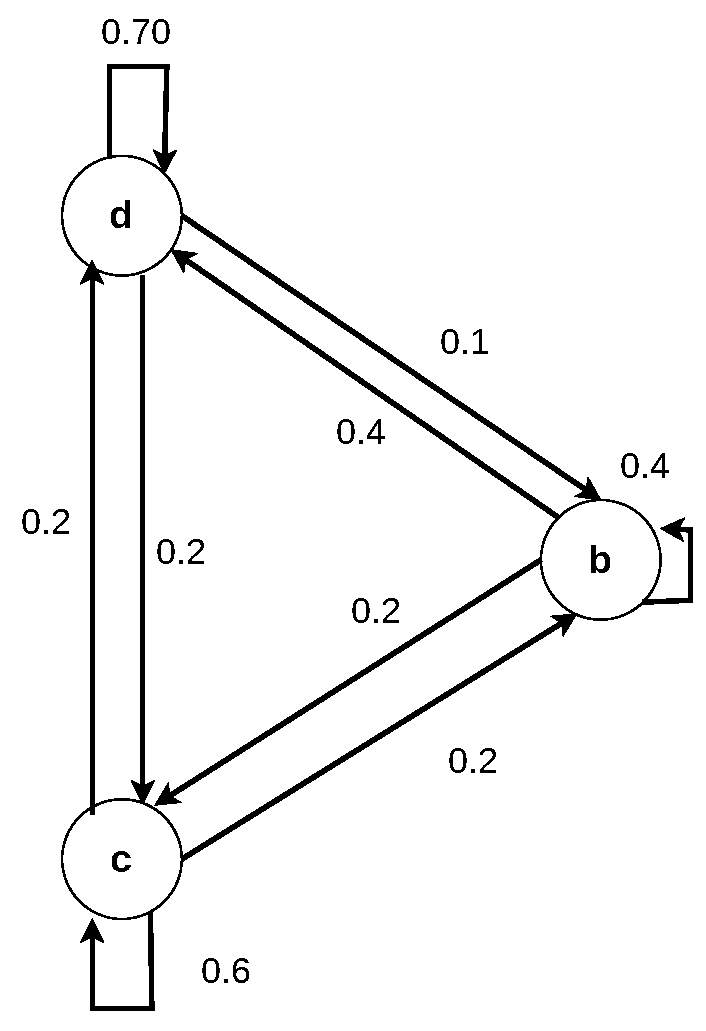
\includegraphics[scale=0.5]{images/markov_cuatro.pdf}
			\end{figure}
		\end{column}
		\begin{column}{0.5\textwidth}
			Para tiempos futuros
			\[P(X_t) = TP(X_{t-1})\equiv P_t\]
			
			\[P1 = TP_0\]
			\[P2 = TP_1\]
			
			\[\begin{bmatrix}
			0.7 & 0.4 & 0.2\\
			0.1 & 0.4 & 0.2\\
			0.2 & 0.2 & 0.6
			\end{bmatrix} \begin{bmatrix}
						0.7 \\
						0.2 \\
						0.1
					  \end{bmatrix}\]
					  
			\[= 					  
			\begin{bmatrix}
						0.57 \\
						0.15 \\
						0.28
					  \end{bmatrix}		 \]
					  
			\[TTP_0=T^2P_0\]
		\end{column}

	\end{columns}
	
\end{frame}

\begin{frame}\small
	\begin{columns}
		\begin{column}{0.5\textwidth}
			\vspace{-0.5cm}
			\begin{figure}
				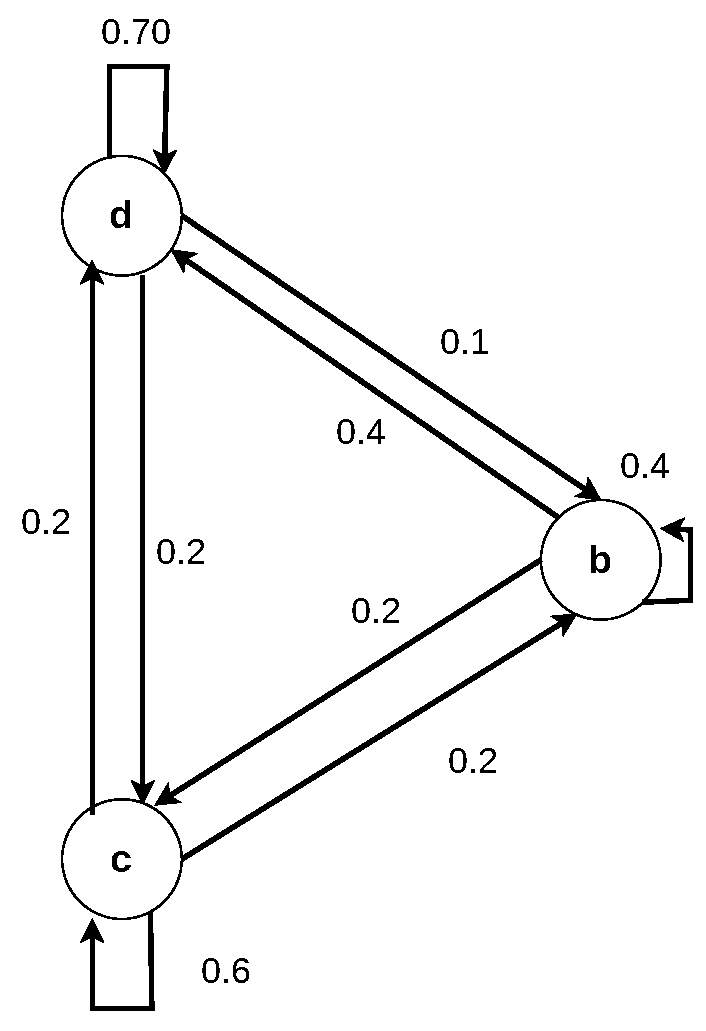
\includegraphics[scale=0.5]{images/markov_cuatro.pdf}
			\end{figure}
		\end{column}
		\begin{column}{0.5\textwidth}
			Para tiempos futuros
			\[P_t = T^tP_0\]

		\end{column}

	\end{columns}
	
\end{frame}


%%%%%%%%%%%%%%%%%%%%%%%%%%%%%%%%%%%%%%%%%%%%%%%%%%%%%%%%%%%%%%%%%%%%%%%%%%%%%%%%%%%%%%%%%%%%
\begin{frame}{Algoritmo de Metropolis \citep{THEODORIDIS20201}}

\begin{itemize}
	\item La distribución propuesta cambia con el tiempo siguiendo la evolución de una cadena de Markov.
	\item La cadena se construye de manera que su matriz de transición tenga la distribución deseada $p(x)$ la cual es invariante. 
	\item La distribución propuesta depende del valor del estado previo,$x_{n-1}$, esto es, $q(\cdot|x_{n-1}) $.
	\item Es decir, generar una nueva muestra (un nuevo estado) depende del valor del estado previo.
\end{itemize}
\end{frame}


\begin{frame}\scriptsize

\begin{algorithm}[H]
	\LinesNumberedHidden
    \begin{algorithmic}
	\STATE{Sea la distribución deseada $p(\cdot)$}
	\STATE{Escoge una distribución de propuesta $q(\cdot|\cdot)$}
	\STATE{Escoge el valor del estado inicial $x_0$}
	\STATE{}
	\FOR{$n = 1,2,\dots, N$ } 
		\STATE{Toma un valor $x \sim q(\cdot | x_{n-1})$}
		\STATE{Calcula el valor de aceptación}
		\STATE{}
		%\STATE{$\alpha (x|x_{n-1}) = \min \Big\lbrace 1,\dfrac{q(x_{n-1}|x)p(x)}{q(x|x_{n-1})p(x_{n-1})} \Big\rbrace$}
			
	\tcc{\scriptsize Si la probabilidad de $p(x)$ es más grande que la de $p(x_{n-1})$, entonces se acepta la nueva muestra. En caso contrario, esta es aceptada-rechazada en base a su valor relativo}
		\STATE{$\alpha (x|x_{n-1}) = \min \Big\lbrace 1,\dfrac{p(x)}{p(x_{n-1})} \Big\rbrace$}
		\STATE{}
		\STATE{Escoge $u \sim U(0,1)$}
		\STATE{}
		\IF{$u \leq \alpha (x|x_{n-1})$}	
			\STATE{$x_n = x$}
		\ELSE
			\STATE{$x_n = x_{n-1}$}
		\ENDIF
	 \ENDFOR
	 	\STATE{}

	\end{algorithmic}
	
\caption{Algoritmo Metropolis \citep{THEODORIDIS20201}}
\end{algorithm}

\end{frame}

\begin{frame}{Turing}
\textbf{Turing} es un lenguaje de programación probabilística de propósito general para una inferencia bayesiana robusta y eficiente. Las características actuales incluyen:

	\begin{itemize}
		\item Programación probabilística de propósito general con una interfaz de modelado intuitiva;
		\item Muestreo de Monte Carlo hamiltoniano (HMC) robusto y eficiente para distribuciones posteriores diferenciables;
		\item 
Muestreo de partículas MCMC para distribuciones posteriores complejas que involucran variables discretas y flujo de control estocástico; e
		\item 
Inferencia composicional a través del muestreo de Gibbs que combina partículas MCMC, HMC y paseo aleatorio MH (RWMH).
	\end{itemize}
\end{frame}

%%%%%%%%%%%%%%%%%%%%%%%%%%%%%%%%%%%%%%%%%%%%%%%%%%%%%%%%%%%%%%%%%%%%%%%%%%%%%%%%%%%%%%%%%%%%


\begin{frame}
	\begin{center}
		{\huge \textbf{¡Vamos a programar!}}
	\end{center}
\end{frame}


\begin{frame}
	\begin{figure}
		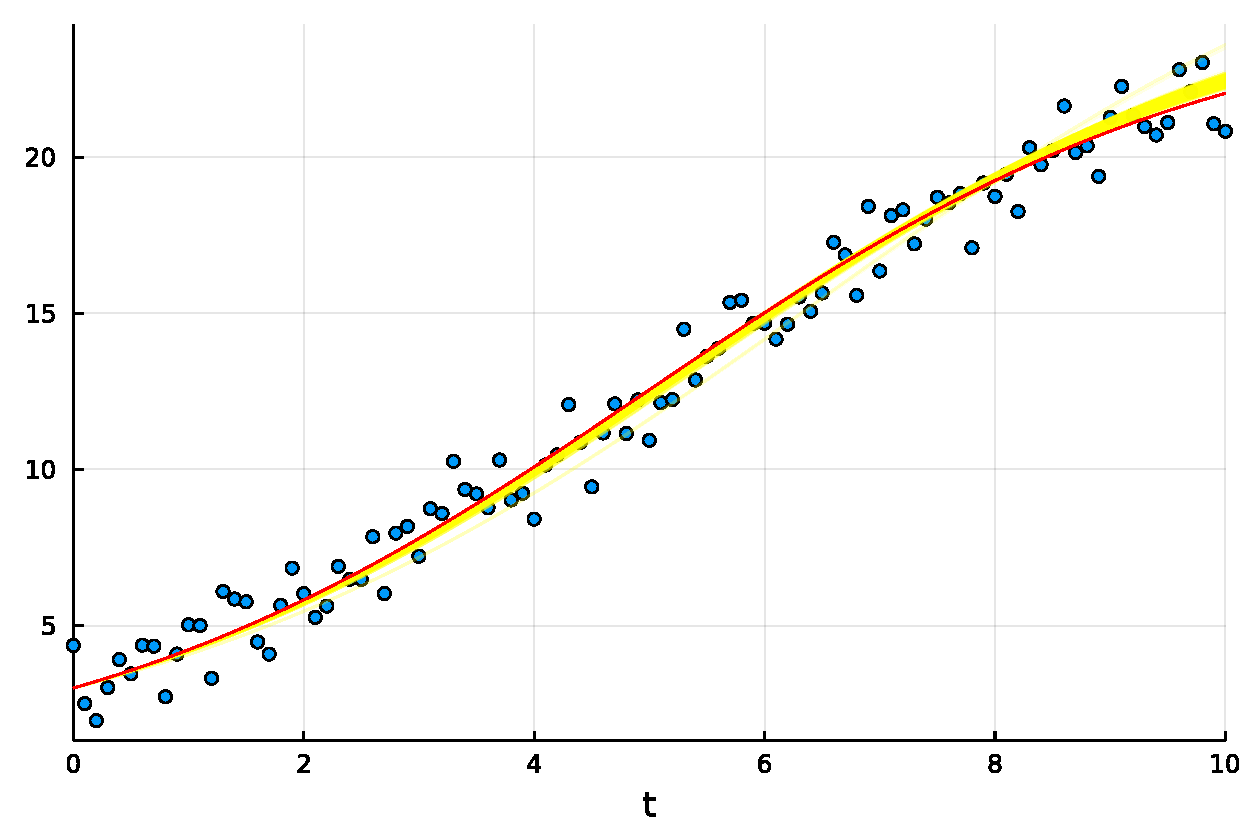
\includegraphics[scale=0.5]{images/final_plot.pdf}
	\end{figure}
	La distribución posterior (línea amarilla) reproduce con bastante precisión la solución \textit{verdadera} del ODE.
\end{frame}

\begin{frame}
	\begin{figure}
		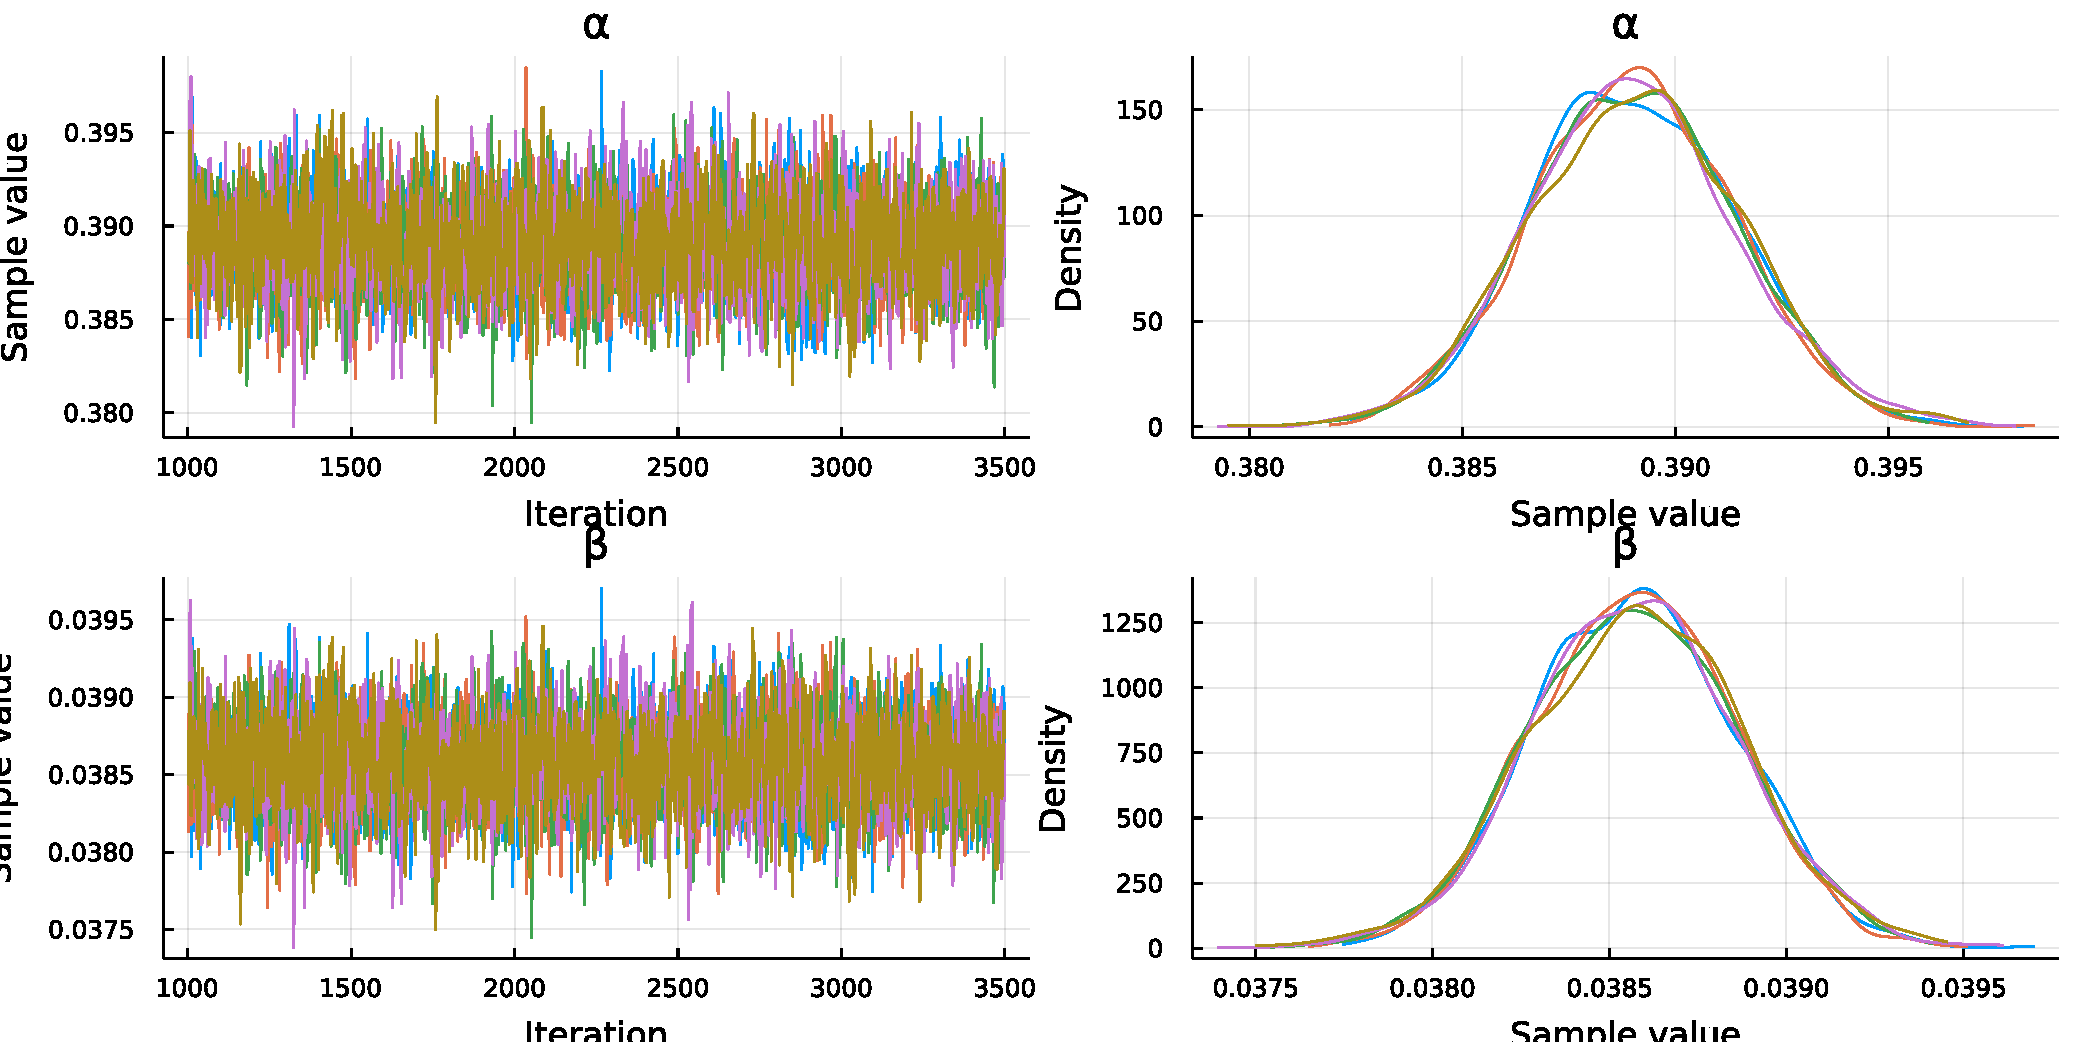
\includegraphics[scale=0.35]{images/chain_resultados.pdf}
	\end{figure}
\end{frame}

\begin{frame}[allowframebreaks]
        \frametitle{References}
		\bibliographystyle{apalike}

       \bibliography{turing_ode.bib}
\end{frame}

\end{document}